\documentclass[a4paper,14pt,oneside,openany]{memoir}

%%% Задаем поля, отступы и межстрочный интервал %%%

\usepackage[left=30mm, right=15mm, top=20mm, bottom=20mm]{geometry} % Пакет geometry с аргументами для определения полей
\pagestyle{plain} % Убираем стандарные для данного класса верхние колонтитулы с заголовком текущей главы, оставляем только номер страницы снизу по центру
\parindent=1.25cm % Абзацный отступ 1.25 см, приблизительно равно пяти знакам, как по ГОСТ
\usepackage{indentfirst} % Добавляем отступ к первому абзацу
%\linespread{1.3} % Межстрочный интервал (наиболее близко к вордовскому полуторному) - тут вместо этого используется команда OnehalfSpacing*

%%% Задаем языковые параметры и шрифт %%%

\usepackage[english, russian]{babel}                % Настройки для русского языка как основного в тексте
\babelfont{rm}{Times New Roman}                     % TMR в качестве базового roman-щрифта

%%% Задаем стиль заголовков и подзаголовков в тексте %%%

\setsecnumdepth{subsection} % Номера разделов считать до третьего уровня включительно, т.е. нумеруются только главы, секции, подсекции
\renewcommand*{\chapterheadstart}{} % Переопределяем команду, задающую отступ над заголовком, чтобы отступа не было
\renewcommand*{\printchaptername}{} % Переопределяем команду, печатающую слово "Глава", чтобы оно не печалось
%\renewcommand*{\printchapternum}{} % То же самое для номера главы - тут не надо, номер главы оставляем
\renewcommand*{\chapnumfont}{\normalfont\bfseries} % Меняем стиль шрифта для номера главы: нормальный размер, полужирный
\renewcommand*{\afterchapternum}{\hspace{1em}} % Меняем разделитель между номером главы и названием
\renewcommand*{\printchaptertitle}{\normalfont\bfseries\centering\MakeUppercase} % Меняем стиль написания для заголовка главы: нормальный размер, полужирный, центрированный, заглавными буквами
\setbeforesecskip{20pt} % Задаем отступ перед заголовком секции
\setaftersecskip{20pt} % Ставим такой же отступ после заголовка секции
\setsecheadstyle{\raggedright\normalfont\bfseries} % Меняем стиль написания для заголовка секции: выравнивание по правому краю без переносов, нормальный размер, полужирный
\setbeforesubsecskip{20pt} % Задаем отступ перед заголовком подсекции
\setaftersubsecskip{20pt} % Ставим такой же отступ после заголовка подсекции
\setsubsecheadstyle{\raggedright\normalfont\bfseries}  % Меняем стиль написания для заголовка подсекции: выравнивание по правому краю без переносов, нормальный размер, полужирный

%%% Задаем параметры оглавления %%%

\addto\captionsrussian{\renewcommand\contentsname{Содержание}} % Меняем слово "Оглавление" на "Содержание"
\setrmarg{2.55em plus1fil} % Запрещаем переносы слов в оглавлении
%\setlength{\cftbeforechapterskip}{0pt} % Эта команда убирает интервал между заголовками глав - тут не надо, так красивее смотрится
\renewcommand{\aftertoctitle}{\afterchaptertitle \vspace{-\cftbeforechapterskip}} % Делаем отступ между словом "Содержание" и первой строкой таким же, как у заголовков глав
%\renewcommand*{\chapternumberline}[1]{} % Делаем так, чтобы номер главы не печатался - тут не надо
\renewcommand*{\cftchapternumwidth}{1.5em} % Ставим подходящий по размеру разделитель между номером главы и самим заголовком
\renewcommand*{\cftchapterfont}{\normalfont\MakeUppercase} % Названия глав обычным шрифтом заглавными буквами
\renewcommand*{\cftchapterpagefont}{\normalfont} % Номера страниц обычным шрифтом
\renewcommand*{\cftchapterdotsep}{\cftdotsep} % Делаем точки до номера страницы после названий глав
\renewcommand*{\cftdotsep}{1} % Задаем расстояние между точками
\renewcommand*{\cftchapterleader}{\cftdotfill{\cftchapterdotsep}} % Делаем точки стандартной формы (по умолчанию они "жирные")
\maxtocdepth{subsection} % В оглавление попадают только разделы первыхтрех уровней: главы, секции и подсекции

%%% Выравнивание и переносы %%%

%% http://tex.stackexchange.com/questions/241343/what-is-the-meaning-of-fussy-sloppy-emergencystretch-tolerance-hbadness
%% http://www.latex-community.org/forum/viewtopic.php?p=70342#p70342
\tolerance 1414
\hbadness 1414
\emergencystretch 1.5em                             % В случае проблем регулировать в первую очередь
\hfuzz 0.3pt
\vfuzz \hfuzz
%\dbottom
%\sloppy                                            % Избавляемся от переполнений
\clubpenalty=10000                                  % Запрещаем разрыв страницы после первой строки абзаца
\widowpenalty=10000                                 % Запрещаем разрыв страницы после последней строки абзаца
\brokenpenalty=4991                                 % Ограничение на разрыв страницы, если строка заканчивается переносом

%%% Объясняем компилятору, какие буквы русского алфавита можно использовать в перечислениях (подрисунках и нумерованных списках) %%%
%%% По ГОСТ нельзя использовать буквы ё, з, й, о, ч, ь, ы, ъ %%%
%%% Здесь также переопределены заглавные буквы, хотя в принципе они в документе не используются %%%

\makeatletter
    \def\russian@Alph#1{\ifcase#1\or
       А\or Б\or В\or Г\or Д\or Е\or Ж\or
       И\or К\or Л\or М\or Н\or
       П\or Р\or С\or Т\or У\or Ф\or Х\or
       Ц\or Ш\or Щ\or Э\or Ю\or Я\else\xpg@ill@value{#1}{russian@Alph}\fi}
    \def\russian@alph#1{\ifcase#1\or
       а\or б\or в\or г\or д\or е\or ж\or
       и\or к\or л\or м\or н\or
       п\or р\or с\or т\or у\or ф\or х\or
       ц\or ш\or щ\or э\or ю\or я\else\xpg@ill@value{#1}{russian@alph}\fi}
\makeatother

%%% Задаем параметры оформления рисунков и таблиц %%%

\usepackage{graphicx, caption, subcaption} % Подгружаем пакеты для работы с графикой и настройки подписей
\graphicspath{{images/}} % Определяем папку с рисунками
\captionsetup[figure]{font=small, width=\textwidth, name=Рисунок, justification=centering} % Задаем параметры подписей к рисункам: маленький шрифт (в данном случае 12pt), ширина равна ширине текста, полнотекстовая надпись "Рисунок", выравнивание по центру
\captionsetup[subfigure]{font=small} % Индексы подрисунков а), б) и так далее тоже шрифтом 12pt (по умолчанию делает еще меньше)
\captionsetup[table]{singlelinecheck=false,font=small,width=\textwidth,justification=justified} % Задаем параметры подписей к таблицам: запрещаем переносы, маленький шрифт (в данном случае 12pt), ширина равна ширине текста, выравнивание по ширине
\captiondelim{ --- } % Разделителем между номером рисунка/таблицы и текстом в подписи является длинное тире
\setkeys{Gin}{width=\textwidth} % По умолчанию размер всех добавляемых рисунков будет подгоняться под ширину текста
\renewcommand{\thesubfigure}{\asbuk{subfigure}} % Нумерация подрисунков строчными буквами кириллицы
%\setlength{\abovecaptionskip}{0pt} % Отбивка над подписью - тут не меняем
%\setlength{\belowcaptionskip}{0pt} % Отбивка под подписью - тут не меняем
\usepackage[section]{placeins} % Объекты типа float (рисунки/таблицы) не вылезают за границы секциии, в которой они объявлены

%%% Задаем параметры ссылок и гиперссылок %%% 

\usepackage{hyperref}                               % Подгружаем нужный пакет
\hypersetup{
    colorlinks=true,                                % Все ссылки и гиперссылки цветные
    linktoc=all,                                    % В оглавлении ссылки подключатся для всех отображаемых уровней
    linktocpage=true,                               % Ссылка - только номер страницы, а не весь заголовок (так выглядит аккуратнее)
    linkcolor=black,                                  % Цвет ссылок и гиперссылок - черный
    citecolor=black                                   % Цвет цитировний - черный
}

%%% Настраиваем отображение списков %%%

\usepackage{enumitem}                               % Подгружаем пакет для гибкой настройки списков
\renewcommand*{\labelitemi}{\normalfont{--}}        % В ненумерованных списках для пунктов используем короткое тире
\makeatletter
    \AddEnumerateCounter{\asbuk}{\russian@alph}     % Объясняем пакету enumitem, как использовать asbuk
\makeatother
\renewcommand{\labelenumii}{\asbuk{enumii})}        % Кириллица для второго уровня нумерации
\renewcommand{\labelenumiii}{\arabic{enumiii})}     % Арабские цифры для третьего уровня нумерации
\setlist{noitemsep, leftmargin=*}                   % Убираем интервалы между пунками одного уровня в списке
\setlist[1]{labelindent=\parindent}                 % Отступ у пунктов списка равен абзацному отступу
\setlist[2]{leftmargin=\parindent}                  % Плюс еще один такой же отступ для следующего уровня
\setlist[3]{leftmargin=\parindent}                  % И еще один для третьего уровня

%%% Счетчики для нумерации объектов %%%

\counterwithout{figure}{chapter}                    % Сквозная нумерация рисунков по документу
\counterwithout{equation}{chapter}                  % Сквозная нумерация математических выражений по документу
\counterwithout{table}{chapter}                     % Сквозная нумерация таблиц по документу

%%% Реализация библиографии пакетами biblatex и biblatex-gost с использованием движка biber %%%

\usepackage{csquotes} % Пакет для оформления сложных блоков цитирования (biblatex рекомендует его подключать)
\usepackage[%
backend=biber,                                      % Движок
bibencoding=utf8,                                   % Кодировка bib-файла
sorting=none,                                       % Настройка сортировки списка литературы
style=gost-numeric,                                 % Стиль цитирования и библиографии по ГОСТ
language=auto,                                      % Язык для каждой библиографической записи задается отдельно
autolang=other,                                     % Поддержка многоязычной библиографии
sortcites=true,                                     % Если в квадратных скобках несколько ссылок, то отображаться будут отсортированно
movenames=false,                                    % Не перемещать имена, они всегда в начале библиографической записи
maxnames=5,                                         % Максимальное отображаемое число авторов
minnames=3,                                         % До скольки сокращать число авторов, если их больше максимума
doi=false,                                          % Не отображать ссылки на DOI
isbn=false,                                         % Не показывать ISBN, ISSN, ISRN
]{biblatex}[2016/09/17]
\DeclareDelimFormat{bibinitdelim}{}                 % Убираем пробел между инициалами (Иванов И.И. вместо Иванов И. И.)
\addbibresource{biba.bib}                           % Определяем файл с библиографией

%%% Скрипт, который автоматически подбирает язык (и, следовательно, формат) для каждой библиографической записи %%%
%%% Если в названии работы есть кириллица - меняем значение поля langid на russian %%%
%%% Все оставшиеся пустые места в поле langid заменяем на english %%%

\DeclareSourcemap{
  \maps[datatype=bibtex]{
    \map{
        \step[fieldsource=title, match=\regexp{^\P{Cyrillic}*\p{Cyrillic}.*}, final]
        \step[fieldset=langid, fieldvalue={russian}]
    }
    \map{
        \step[fieldset=langid, fieldvalue={english}]
    }
  }
}

%%% Прочие пакеты для расширения функционала %%%

\usepackage{longtable,ltcaption}                    % Длинные таблицы
\usepackage{multirow,makecell}                      % Улучшенное форматирование таблиц
\usepackage{booktabs}                               % Еще один пакет для красивых таблиц
\usepackage{soulutf8}                               % Поддержка переносоустойчивых подчёркиваний и зачёркиваний
\usepackage{icomma}                                 % Запятая в десятичных дробях
\usepackage{hyphenat}                               % Для красивых переносов
\usepackage{textcomp}                               % Поддержка "сложных" печатных символов типа значков иены, копирайта и т.д.
\usepackage[version=4]{mhchem}                      % Красивые химические уравнения
\usepackage{amsmath}                                % Усовершенствование отображения математических выражений 

%%% Мои (Дениса) плагины %%%

\usepackage{cmap}					% поиск в PDF
\usepackage{listings}
\usepackage{xcolor}
\usepackage{matlab-prettifier}
\usepackage{pgfplots}

%%% Listing styling

\lstdefinestyle{myCustomMatlabStyle}{
  language=Matlab,
  numbers=left,
  stepnumber=1,
  numbersep=10pt,
  tabsize=4,
  showspaces=false,
  showstringspaces=false
}

% A "tiny" listing
\lstset{basicstyle=\tiny,style=myCustomMatlabStyle, extendedchars=\true, texcl=true}

%%% Вставляем по очереди все содержательные части документа %%%


\begin{document}

\thispagestyle{empty}

\begin{center}
    МИНИСТЕРСТВО НАУКИ И ВЫСШЕГО ОБРАЗОВАНИЯ \\ РОССИЙСКОЙ ФЕДЕРАЦИИ

    \vspace{20pt}

    Санкт-Петербургский политехнический университет Петра Великого \\ Институт компьютерных наук и кибербезопасности \\
    Высшая школа интеллектуальных систем и суперкомпьютерных технологий \\

    \vspace{20pt}

\end{center}

\vfill

\begin{center}
    ОТЧЕТ \\  
    по производственной практике \\

    \vspace{20pt}

    по теме: \\
    \uppercase{Алгоритмы сжатия с потерями}
\end{center}

\vfill

    \noindent Студент: \\
    \textit{Группа № 5140901/31501 \hfill Д.С. Кузик}

    \vspace{20pt}

    \noindent Руководитель: \\
    \textit{доцент \hfill К.К. Семенов}

\vfill

\begin{center}
    Санкт-Петербург\\
    2024
\end{center}                                     % Титульник

\newpage % Переходим на новую страницу
\setcounter{page}{2} % Начинаем считать номера страниц со второй
\OnehalfSpacing* % Задаем полуторный интервал текста (в титульнике одинарный, поэтому команда стоит после него)

\tableofcontents*                                   % Автособираемое оглавление

\chapter{Постановка задачи}
\label{ch:intro}

Задача 9.

Выполнить анализ алгоритмов сжатия с потерями KRLE (K-Run Length Encoding), LTC
(Lightweight Coding) и метрологического JPEG. Выполнить описание данных алгоритмов.
Реализовать данные алгоритмы в пакете Matlab и на языке Python. Выполнить тестирование.
Выполнить сравнительный анализ.

\endinput                                     % Введение
\chapter{Описание алгоритмов}
\label{ch:chap1}

\section{K-RLE}

В контексте использования технологии беспроводной сенсорной сети
(WSN) для мониторинга окружающей среды двумя
основными элементарными функциями WSN являются сбор
и передача данных. Однако передача/прием данных
требует больших затрат энергии. Чтобы снизить энергопотребление, связанное с передачей, используется сжатие данных с помощью локальной обработки информации.

Рассмотрим новый алгоритм сжатия данных, основанный на кодировании длины выполнения (RLE), который называется K-RLE.

Идея, лежащая в основе этого нового алгоритма, заключается в следующем:
пусть $K$ - число, если элемент данных $d$, $d+K$ или $d-K$ встречается n раз подряд во входном потоке, мы заменяем эти n вхождений
одной парой $nd$ \cite{krle_article}.

\begin{figure}[ht]
    \centering
    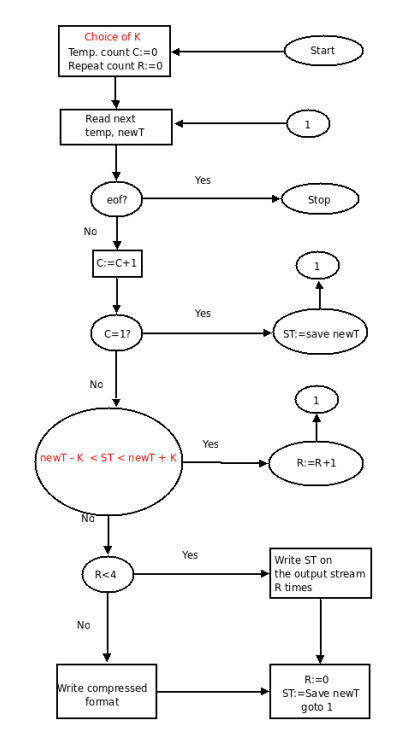
\includegraphics[width=0.5\textwidth]{krle_alg.png}
    \caption{K-RLE Алгоритм}
    \label{fig:krle_alg}
\end{figure}

\endinput                                     % Первая глава
\chapter{Разработанный код}
\label{ch:chap2}

Исходный код на GitHub:

https://github.com/Denisqu/masters-practice-sem2

\section{K-RLE}

Представим разработанные алгоритмы кодирования и декодирования K-RLE на языке программирования Python:

\begin{lstlisting}[language=python, caption=K-RLE реализация на языке Python, captionpos=b, frame=single]
    from typing import List

    def k_rle_code(stream: List[int], K: int) -> List[int]:
        # Функция для кодирования потока чисел с использованием модифицированного RLE алгоритма.
        # 
        # Алгоритм:
        # 1. Проходим по входному потоку чисел.
        # 2. Если элемент повторяется (учитывая допустимое отклонение K), увеличиваем счетчик повторов.
        # 3. Если элемент не повторяется, вставляем текущие накопленные повторы в результат.
        # 4. В конце вставляем оставшиеся элементы после завершения цикла.
        # 
        # Аргументы:
        # stream -- входной поток чисел
        # K -- допустимое отклонение для повторяющихся чисел
        # 
        # Возвращает:
        # Закодированный поток чисел

        result_stream = []
        count = 0
        repeat_count = 0
        ST = 0
        
        def insert_func():
            if repeat_count < 4:
                result_stream.extend([ST] * (repeat_count + 1))
            else:
                result_stream.extend([repeat_count, ST])
        
        for i, newT in enumerate(stream):
            count += 1
            if count == 1:
                ST = newT
                continue
            if (newT + K > ST and newT - K < ST) or newT == ST:
                repeat_count += 1
                continue
            insert_func()
            repeat_count = 0
            ST = newT
        insert_func()
            
        return result_stream
    
    def k_rle_decode(stream: List[int], threshold: int) -> List[int]:
        # Функция для декодирования потока чисел, закодированного модифицированным RLE алгоритмом.
        #
        # Алгоритм:
        # 1. Проходим по входному закодированному потоку чисел.
        # 2. Если элемент меньше порога и больше 0, считаем его как количество повторов и добавляем соответствующие элементы в результат.
        # 3. Если элемент не является счетчиком повторов, просто добавляем его в результат.
        # 4. Переходим к следующему элементу.
        #
        # Аргументы:
        # stream -- входной закодированный поток чисел
        # threshold -- порог для определения счетчиков повторов
        #
        # Возвращает:
        # Декодированный поток чисел
        
        result_stream = []
        i = 0
        while i < len(stream):
            if stream[i] < threshold and stream[i] > 0:
                result_stream.extend([stream[i+1]] * (stream[i] + 1))
                i += 2
            else:
                current = stream[i]
                result_stream.append(current)
                i += 1
        return result_stream
    
\end{lstlisting}

\section{LTC}

Представим разработанный алгоритм кодирования
LTC на языке программирования Python:

\begin{lstlisting}[language=python, caption=ltc реализация на языке Python, captionpos=b, frame=single]

    from typing import List, Tuple

    def ltc_code(data_stream: List[Tuple[int, int]], e: int) -> List[Tuple[int, int]]:
        # Алгоритм:
        # 1. Инициализация: получение первой точки данных, сохранение её в z. Получение следующей точки (t2, v2),
        #    использование её для инициализации границ UL (верхняя граница) и LL (нижняя граница).
        # 2. Вычисление highLine как линии, соединяющей z и UL.
        # 3. Вычисление lowLine как линии, соединяющей z и LL.
        # 4. Получение следующей точки данных. Преобразование точки в вертикальный сегмент с использованием погрешности e.
        #    Определение ul как верхней точки сегмента и ll как нижней точки сегмента.
        # 5. Если highLine находится ниже ll или lowLine находится выше ul, переход к шагу 9, иначе продолжение.
        # 6. Если highLine выше ul, установка UL в ul.
        # 7. Если lowLine ниже ll, установка LL в ll.
        # 8. Переход к шагу 2.
        # 9. Завершение: вывод z в выходной поток данных.
        # 10. Установка z как точки, находящейся посередине между UL и LL.
        # 11. Установка UL как ul.
        # 12. Установка LL как ll.
        # 13. Переход к шагу 2.
    
        def calculate_line(p1: Tuple[float, float], p2: Tuple[int, int])
         -> Tuple[int, int]:
            #Вычисляет коэффициенты прямой, проходящей через две точки (p1 и p2)
            x1, y1 = p1
            x2, y2 = p2
            slope = (y2 - y1) / (x2 - x1)
            intercept = y1 - slope * x1
            return slope, intercept
    
        result_stream = []
        z = data_stream[0]
        t2, v2 = data_stream[1]
        UL = (t2, v2 + e)
        LL = (t2, v2 - e)
        i = 2
    
        while i < len(data_stream):
            highLine = calculate_line(z, UL)
            lowLine = calculate_line(z, LL)
            t, v = data_stream[i]
            ul = (t, v + e)
            ll = (t, v - e)
            
            slope_high, intercept_high = highLine
            slope_low, intercept_low = lowLine
            
            if (slope_high * t + intercept_high < ll[1]) 
            or (slope_low * t + intercept_low > ul[1]):
                result_stream.append(z)
                z = ((UL[0] + LL[0]) / 2, (UL[1] + LL[1]) / 2)
                UL = ul
                LL = ll
            else:
                if slope_high * t + intercept_high > ul[1]:
                    UL = ul
                if slope_low * t + intercept_low < ll[1]:
                    LL = ll
    
            i += 1
    
        result_stream.append(z)
        
        return result_stream
\end{lstlisting}


\endinput                                     % Вторая глава
\chapter{Тестирование алгоритмов}

\endinput                                     % Третья глава
\chapter{Анализ результатов и выводы}

\endinput                                     % выводы

\printbibliography[title=Список использованных источников] % Автособираемый список литературы

\end{document}